\scanpage{90}

\[
\text{(24)}\qquad |\lambda_1|\mathord{-}|\lambda_n|=\rho_1\mathord{-}\rho_n
\]

\deleted{Indeed, the \deleted{\unsure{product}}\inserted{square of the first} side is equal to \deleted{$|\lambda_1\unsure{\rho|q}$} $|\lambda_1\mathord{\cdot}\,\mathord{-}\lambda_n|^2=|\det u|^2=(\overline{\det u},\unsure{\overset{\deleted{\mathrm{conj}}}{\det u}|\overline{\det u}})=(\det u^*)\det u\deleted{{}^{\unsure{*}}}=\det u^*u=\rho_1^2\mathord{-}\,\mathord{-}\rho_n^2$, where $\rho_1\mathord{-}\rho_n$ are the eigenvalues of $(u^*u)^{1/2}$, whence (23).}
\textcolor{red}{\uline{\textcolor{black}{It \deleted{\unsure{that}} \inserted{\deleted{\unsure{whence}}} follows, \unsure{thus|then},}}}

\reversemarginpar
\margin{We have \deleted{\unsure{on the other|on the one hand} $\unsure{\lambda_1}\mathord{-}\lambda_n=\det\inserted{\deleted{\unsure{u}}}$}
\begingroup\setbox0=\hbox{$\text{(25)}\quad\lambda_1(u)\mathord{-}\lambda_n(u)=\det u$}\dimen0=\wd0\advance\dimen0 by6pt\dimen2=\ht0\advance\dimen2 by3pt\dimen4=\dp0\advance\dimen4 by3pt\dimen6=\dimen4\advance\dimen6 by-2pt\leavevmode\hspace{3pt}\rlap{\begin{tikzpicture}[overlay,baseline=0pt]\draw[line width=.45pt] (-3pt,\the\dimen2)--(-3pt,-\the\dimen4)--(\the\wd0,-\the\dimen4);\draw[line width=.45pt] (\the\dimen0,-\the\dimen6)--(\the\dimen0,\the\dimen2);\end{tikzpicture}}\box0\hspace{6pt}\endgroup
\deleted{and on} on the other hand $(\rho_1(u)\mathord{-}\rho_n(u))^2=\rho_1(u^*u)\mathord{\cdot}\,\mathord{-}\rho_n(u^*u)=\det(u^*u)=\det u^*\,\det u=\overline{\det u}\det u=|\det u|^2$, whence
\begingroup\setbox0=\hbox{$\deleted{\unsure{(25)|(24)}}\ \text{\textcircled{26}}\quad\rho_1(u)\mathord{-}\rho_n(u)=\det|u|$}\dimen0=\wd0\advance\dimen0 by3pt\dimen2=\ht0\advance\dimen2 by3pt\dimen4=\dp0\advance\dimen4 by3pt\dimen6=\wd0\divide\dimen6 by10\dimen8=\wd0\advance\dimen8 by-\dimen6\dimen6=\dimen4\advance\dimen6 by-2pt\leavevmode\hspace{3pt}\rlap{\begin{tikzpicture}[overlay,baseline=0pt]\draw[line width=.45pt] (0pt,\the\dimen2)--(\the\dimen0,\the\dimen2);\draw[line width=.45pt] (-3pt,\the\dimen2)--(-3pt,-\the\dimen4)--(\the\dimen0,-\the\dimen4);\draw[line width=.45pt] (\the\dimen8,-\the\dimen4) to[out=70,in=180] (\the\wd0,-\the\dimen6);\end{tikzpicture}}\box0\hspace{3pt}\endgroup
Comparing (25) and (26), \unsure{tr.|t.} $\Rightarrow$ (24)}
\normalmarginpar

when $u$ is invertible, \deleted{that} thus \deleted{$|\lambda_1\mathord{-}\lambda_n|$ \unsure{and}} the $\lambda_i$ and the $\rho_i$ nonzero \deleted{\unsure{that they are}}, that the conditions of \deleted{corollary 1 of fundamental lemma 2 are satisfied, under hypothesis b)} \inserted{\unsure{theorem|Proposition} 1, 2\uuline{°}, hypothesis b are satisfied.} If one supposes that $f$ is moreover \textcolor{red}{\uline{\textcolor{black}{defined}}} and continuous for $r_i\geq0$, since we shall have (23) for \deleted{every} invertible $u$ and the two sides are continuous functions of $u$ as one verifies at once, it follows that the inequality will be satisfied for \deleted{every} $u$. -- The

\deleted{\uline{Corollary 5}} follows for example from corollary 4 that if $u$ is invertible, formulas (21) are satisfied $=$ if $p$ is not positive. Note that \deleted{under the conditions of corollary 3, one deduces from \unsure{(24)|(26)} and the inequalities $|\lambda_1\mathord{-}\lambda_k|\leq\rho_1\mathord{-}\rho_k$, \unsure{the analogous relations}}

\reversemarginpar
\margin{\deleted{\unsure{(25)|(24)|(27)} $|\lambda_k\mathord{-}\lambda_n|\leq\rho_{\unsure{k|n}}\mathord{-}\rho_n$ $(1\leq k\leq n)$, \unsure{which} \illegible{2} for $\unsure{\rho_k}\mathord{-}\unsure{\rho_n}$, \illegible{3} \unsure{the} \illegible{2}} \textcolor{red}{\textcircled{?}}}
\margin{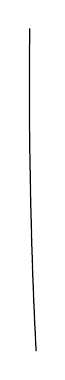
\begin{tikzpicture}[x=1cm,y=1cm]\draw[line width=.45pt] (0,0) .. controls (-.02,-1.05) and (.01,-2.85) .. (.08,-4.1);\end{tikzpicture}}
\normalmarginpar

\uline{Corollary 5} Let $u$ be an operator in a Hilbert space $E$, let $N$ be a Schatten norm on $R^{\deleted{I}\inserted{k}}$, \deleted{where $I=\deleted{\dim}(1,\unsure{\mathord{-}}n)$ \unsure{if} $\dim E=n$, and $I=$ set of integers if} \inserted{where $k\leq\dim E$.} \inserted{Then, we have}

\[
\text{(27)}\qquad N(|\lambda_1|,\mathord{-}\,\mathord{-}|\lambda_k|)\leq N(\rho_1,\mathord{-}\,\mathord{-}\rho_k)
\]

\deleted{Whence, $\unsure{N(}\unsure{\leq|\xi|k|\lambda_i}$} Consequently, if the dimension of $E$ is infinite and if $N$ is a Schatten norm on \deleted{\unsure{all|of}} the space $R^{(\underline N)}$, \deleted{\unsure{when} $\underline N$ \unsure{denotes}} \inserted{we have}

\[
\text{\unsure{(28)|(26)}}\qquad N((|\lambda_i|))\leq N((\rho_i))
\]

In this statement, $\underline N$ denotes the set of integers, hence $R^{(\underline N)}$ the space of sequences of \unsure{real numbers|integers} \deleted{\unsure{which are}} of which only a finite number of terms are nonzero. A norm on $R^{(\underline N)}$ is called a Schatten norm, if it induces a Schatten norm on \deleted{every} a, space $R^n$ (embedded in the natural way in $R^{(\underline N)}$).

\reversemarginpar
\margin{91}
\normalmarginpar
